\documentclass[10pt,a4paper]{article}
\usepackage[utf8]{inputenc}
\usepackage{amsmath}
\usepackage{amsfonts}
\usepackage{amssymb}
\usepackage{graphicx}
\usepackage{multicol}
\usepackage[margin=1in]{geometry}

\title{Makespan Schedule Explanation Questionnaire}
\date{}
\author{}

\begin{document}
\maketitle
\vspace{-4\baselineskip}
\noindent\hrulefill

This questionnaire will judge the general ability to understand and explain makespan schedule. Makespan schedules consist of $m$ machines and $n $ jobs. Every job is assigned to only one machine for the schedule to be feasible. Each job has a processing time. The objective is to minimise the longest collective processing time. Machines and jobs are denoted by integers $1,2,3,...$ and by letters $A,B,C,...$, respectively. A schedule is optimal when the longest collective processing time cannot be faster.

\begin{multicols}{2}
	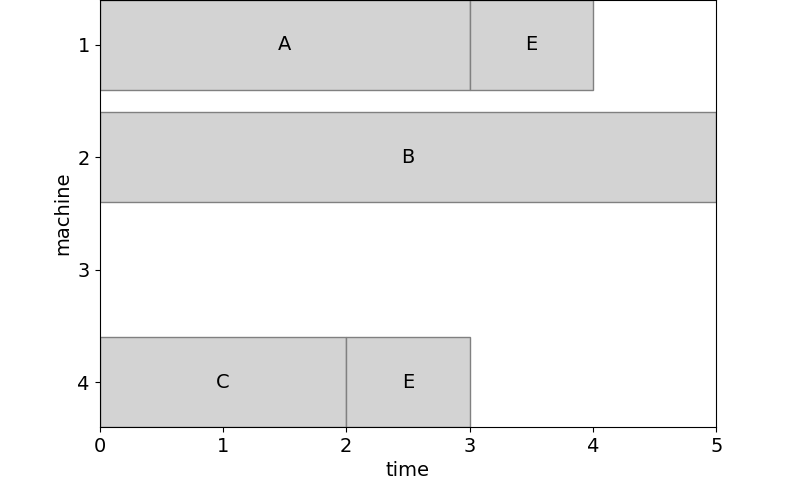
\includegraphics[width=0.5\textwidth]{figures/makespan_infeasible}
	\begin{center}
		Schedule 1: Infeasible because $D$ is not assigned to any machine and $E$ is assigned to multiple machines.
	\end{center}
	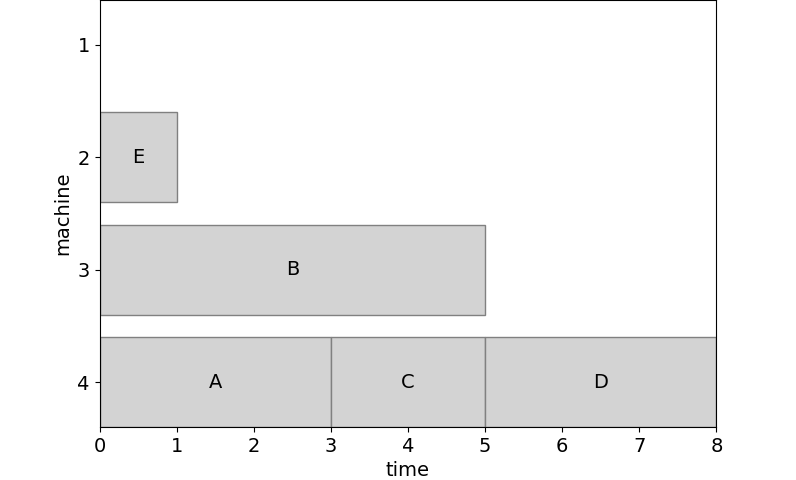
\includegraphics[width=0.5\textwidth]{figures/makespan_unoptimal}
	\begin{center}
		Schedule 2: Non-optimal because jobs $A,C,D$ can be moved to machine $1$.
	\end{center}
\end{multicols}

\vspace{-\baselineskip}
\noindent\hrulefill

Aim to spend at most one minute for each question. Some questions are designed to be difficult.

\begin{enumerate}
	\item Is this schedule optimal? If not, suggest how it could be improved.
	\begin{center}
		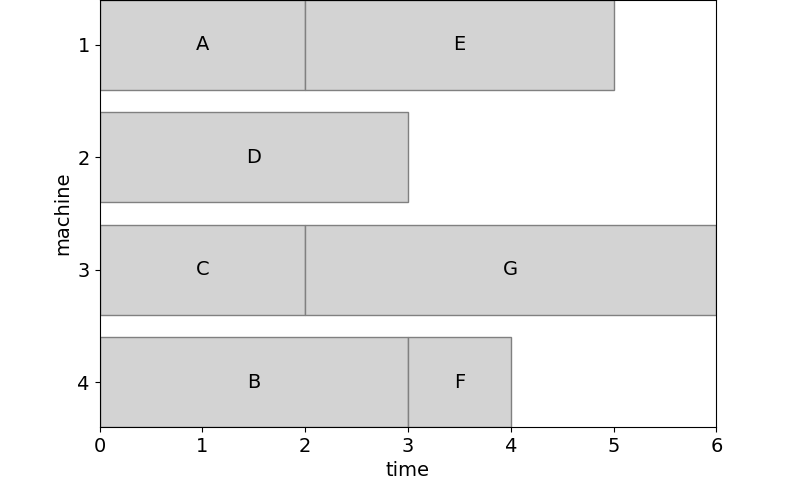
\includegraphics[width=0.5\textwidth]{figures/makespan_question1}
	\end{center}
	\item This schedule is optimal. Suppose that job $A$ cannot be assigned to machine $1$ or $2$ anymore. How could the schedule be modified to agree with this decision?
	\begin{center}
		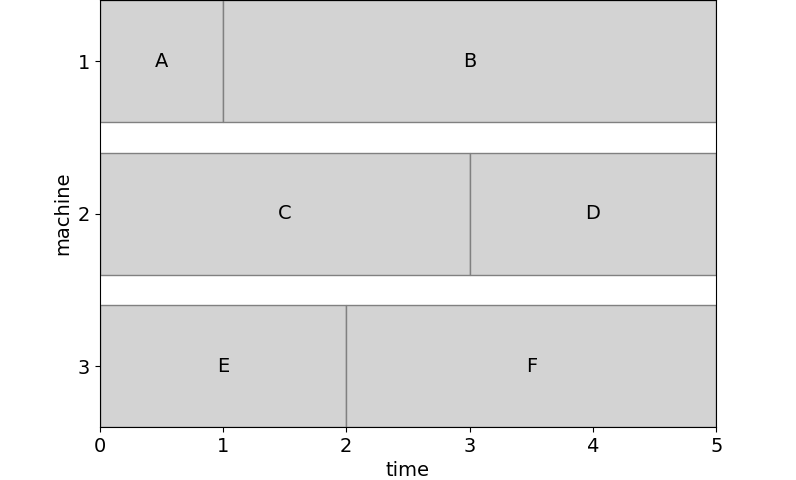
\includegraphics[width=0.5\textwidth]{figures/makespan_question2}
	\end{center}
\end{enumerate}

\end{document}
